\documentclass{beamer}
\usepackage{graphicx}
\usepackage{algorithm2e}
\usepackage{multicol}

\begin{document}

\begin{frame}
\frametitle{Graph Coloring Problem}
\centering{
  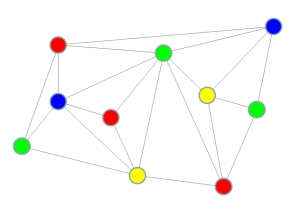
\includegraphics[height=150px]{graph_coloring.jpg}
}
\begin{itemize}
\item Given a Graph $G=(V,E)$, assign a color to each Vertex such that no adjecent vertex has the same color
\item Find the minimum ammount of colors such that the property above holds
\end{itemize}
\end{frame}

\begin{frame}
\frametitle{Graph Coloring Problem}
\large{Formally:}
\begin{itemize}
\item Given an un-directed graph $G=(V,E)$, defined as a set of vertices $V$ and edges $E$, a subset of $V$ is called independent if no two adjacent vertices belong to it.
\item A k-coloring is a partition of $G$ into $k$ independent sets
\item An optimal coloring is the smallest k-coloring possible for a graph
\item Want: An optimal coloring
\end{itemize}
\end{frame}

\begin{frame}
\frametitle{Previous Approaches}
\begin{itemize}
\item {\bf Greedy Constructive Methods:} Succesively choose a vertex and a color such that the independent property holds according to some criteria. Poor performance in general.
\item {\bf Genetic Algorithm:} Ordering of vertices encoded as a coloring and use a GA to optimize. No good performance.
\item {\bf Local Search:} Use simulating annealing or tabu search. Differ from each other in the way they define a neighborhood, cost function and search space. State of the art!
\end{itemize}
\end{frame}

\begin{frame}
\frametitle{Hybrid Algorithms}
\begin{multicols}{2}
\begin{itemize}
\item A configuration $s\ \in\ S$ is any partition $s\ =\ \{V_i,..V_k\}$ of $V$ in $k$ subsets
\item A configuration $s$ might not be a proper k-coloring
\item The cost or penalty of a configuration $s$ is the number of conflicting vertices
\item Main difference between a GA: mutation is replaced by a local search operator
\item Early stop if diversity is low
\end{itemize}
\columnbreak
\small{
\begin{algorithm}[H]
\KwData{graph G = (V,E), integer k}
\KwResult{the best configuration found}
{\bf begin}\;
$P\ =\ InitPopulation(|P|)$\;
\While{not Stop-Condition()}{

  $(s1,s2)\ =\ ChooseParents(P)$\;
  $s\ =\ Crossover(s1,s2)$\;
  $s\ =\ LocalSearch(s,L)$\;
  $P\ =\ UpdatePopulation(P,s)$
}
\end{algorithm}
}
where,
\begin{itemize}
\item $L$ is the number of iterations that the local search will perform
\end{itemize}
\end{multicols}
\end{frame}

\begin{frame}
\frametitle{New Crossover Operator}
\begin{itemize}
\item Generic crossover operators perform badly
\item Domain specific knowledge seems to be necesary for this problem
\item {\bf Assignment Approach:} Child inherits the color of a vertex from a parent with equal probability unless it causes a conflict
\item {\bf Partition Approach:} Childs inherit from the parent color classes or subsets of color classes
\end{itemize}

\end{frame}

\begin{frame}
\frametitle{CPX Crossover Operator}
\begin{multicols}{2}
\begin{itemize}
\item Choose a class from a parent which has maximum coloring
\item Remove the vertices of the class from the classes of the parents
\item Assign randomly the vertices left unassigned
\end{itemize}
\columnbreak
\tiny{
\begin{algorithm}[H]
\KwData{configurations $s_1\ =\ \{V_1^1,...,V_k^1\}$ and $s_2\ =\ \{V_1^2,...,V_k^2\}$}
\KwResult{configuration $s\ =\ \{V_1,...,V_k\}$}
{\bf begin}\;
\For{$l\ =\ 1..k$}{

  \eIf{$l$ is odd}{$A\ =\ 1$}{$A\ =\ 2$}
  choose i such tat $V_i^A$ has maximum cardinality\;
  $V_l\ =\ V_i^A$\;
  remove teh vertices of $V_l$ from $s_1$ and $s_2$\;
}
Assign randomly the vertices of $V\ -\ (V_1\ \cup ... \cup\ V_k)$\;
\end{algorithm}
}
\end{multicols}

\end{frame}

\begin{frame}

\frametitle{Local Search Operator}

\begin{itemize}

\item A neighbor is obtained by moving a vertex to another color class
\item A vertex is only moved if it conflicts with other vertex
\item A tabu move which performs better than the best configuration is always accepted
\item The search is repeated for a specific number of iterations $L$

\end{itemize}

\end{frame}

\begin{frame}
\frametitle{Runnng Profile}
\centering{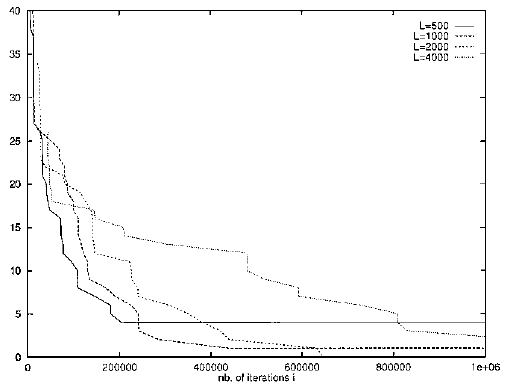
\includegraphics[height=140px]{runProf.png}}
\begin{itemize}
\item {\bf Running Profile:} The best coloring found after a particular number of iterations
\item When $L$ is 500 and 1000, best solution is not found; with 2000 and 4000 best solution is found
\item When $L$ is larger, the search progresses more slowly.
\end{itemize}
\end{frame}

\begin{frame}
\frametitle{Diversity}
\centering{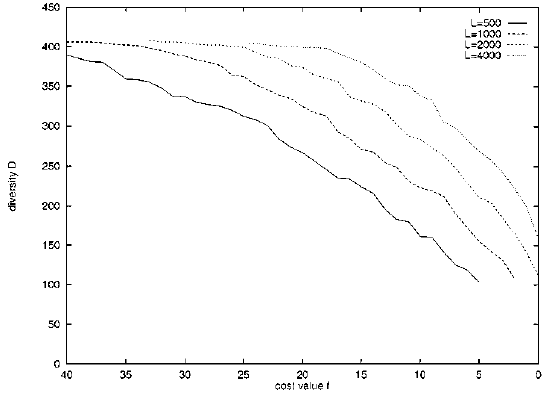
\includegraphics[height=140px]{div.png}}
\begin{itemize}
\item {\bf Difference Function:} Number of transformations to convert one coloring into another 
\item Longer local search sets the children far away from the parents
\end{itemize}
\end{frame}


%% \begin{frame}
%% \frametitle{Comparison with Tabu Search}
%% \centering{
%% 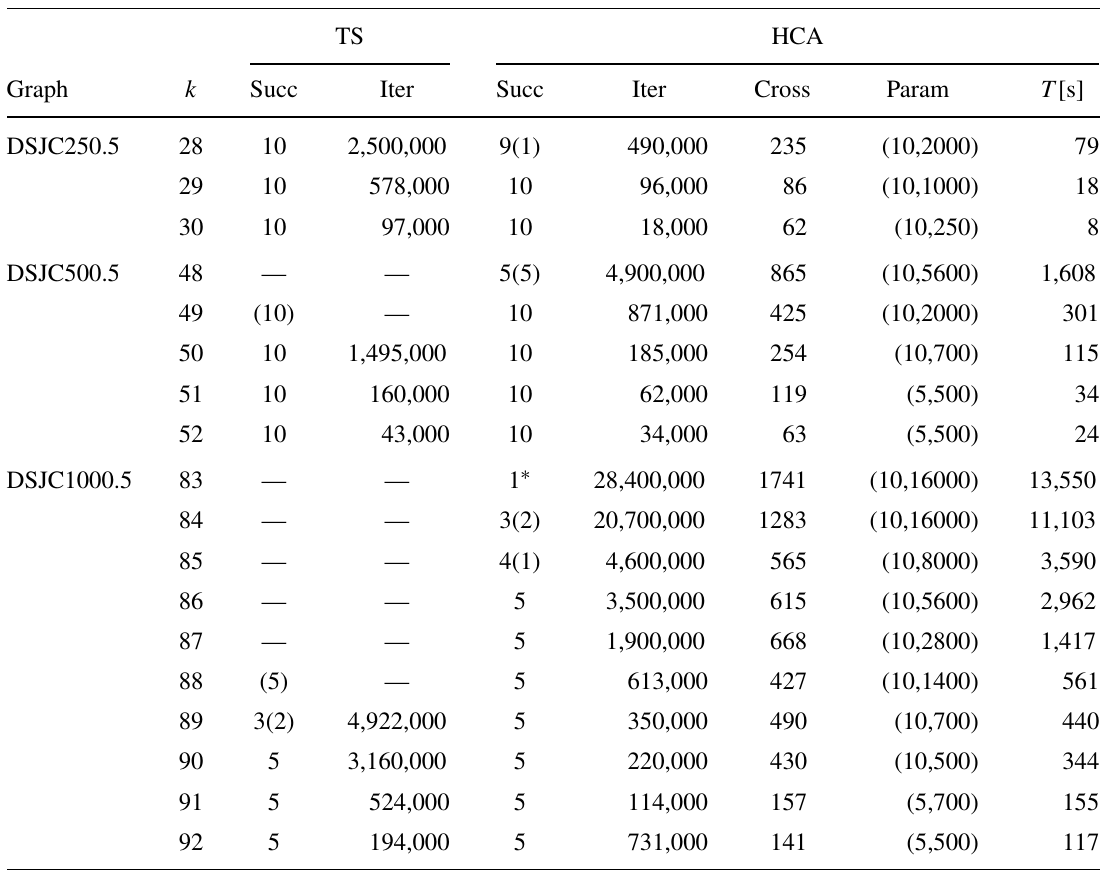
\includegraphics[height=200px]{results1.png}
%% }

%% \end{frame}

%% \begin{frame}

%% \frametitle{Results}
%% \centering{
%% 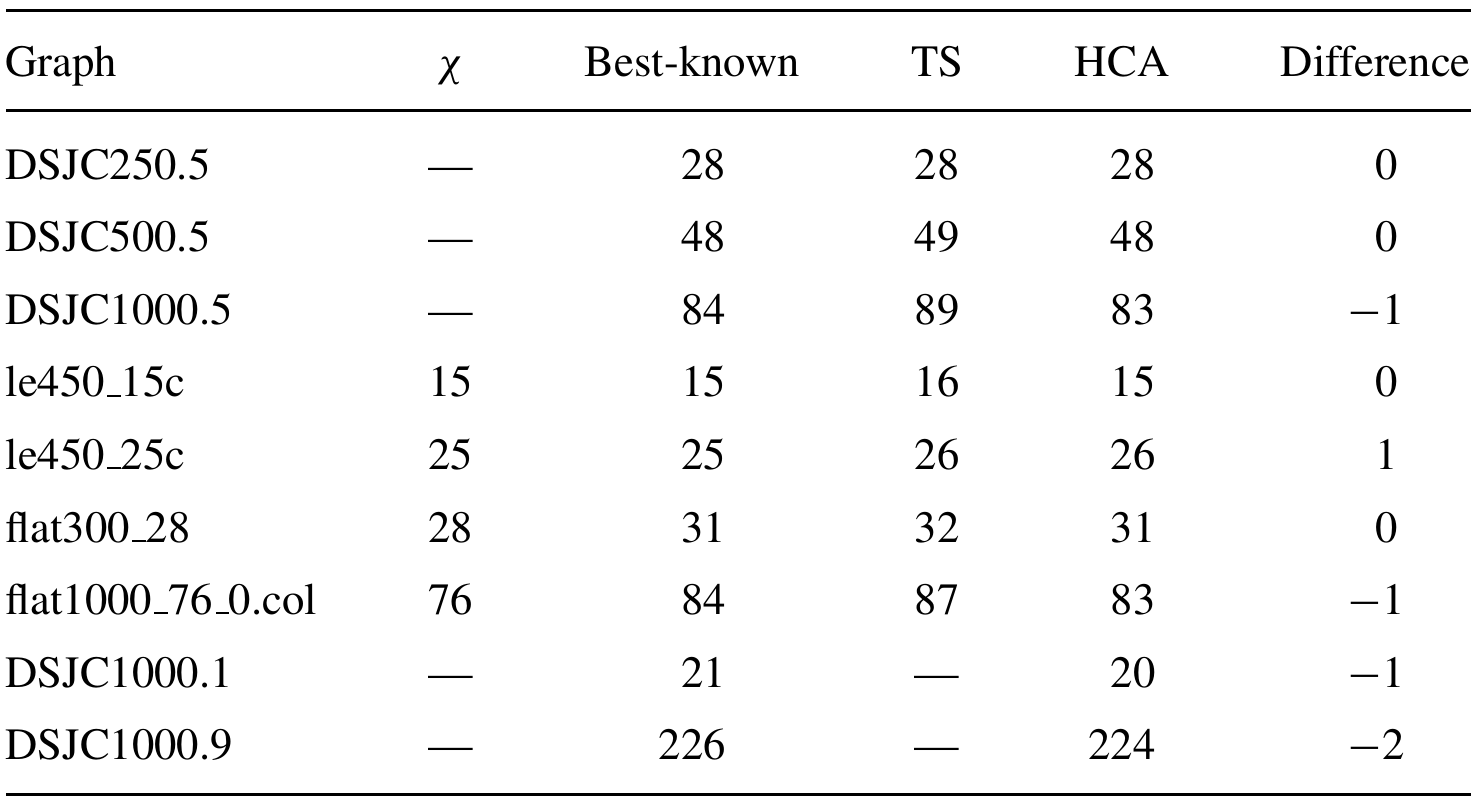
\includegraphics[height=160px]{results2.png}
%% }

%% \end{frame}

\begin{frame}
\frametitle{Conclusions}
%Not completed
\begin{itemize}
\item A domain specific crossover operator is necessary
\item Longer local search is necessary for difficult problems
% \item
\end{itemize}
\end{frame} 

\end{document}
